% Source for fig_4_4_3_st_reservation.pdf (ST-02). Build: pdflatex fig_4_4_3_st_reservation.tex
\documentclass[tikz,border=3pt]{standalone}
\usepackage[T1]{fontenc}\usepackage{lmodern}
\usetikzlibrary{arrows.meta,calc,shapes.geometric}
\newcommand{\diagramfont}{\scriptsize\linespread{1}\selectfont}
\tikzset{
  diagram/.style={x=1mm,y=1mm,font=\diagramfont,>={Stealth[length=1.7mm,width=1.3mm]},line width=0.4pt},
  st/.style={draw,rounded corners=2.5mm,fill=white,minimum width=34mm,minimum height=10mm,align=center,font=\footnotesize\bfseries},
  tl/.style={fill=white,inner sep=0.6mm,align=center,font=\diagramfont},
  ad initial/.style={circle,fill=black,minimum size=3mm,inner sep=0},
  ad final/.style={circle,draw,double,double distance=0.6mm,fill=black,minimum size=2.4mm,inner sep=0}}

\begin{document}
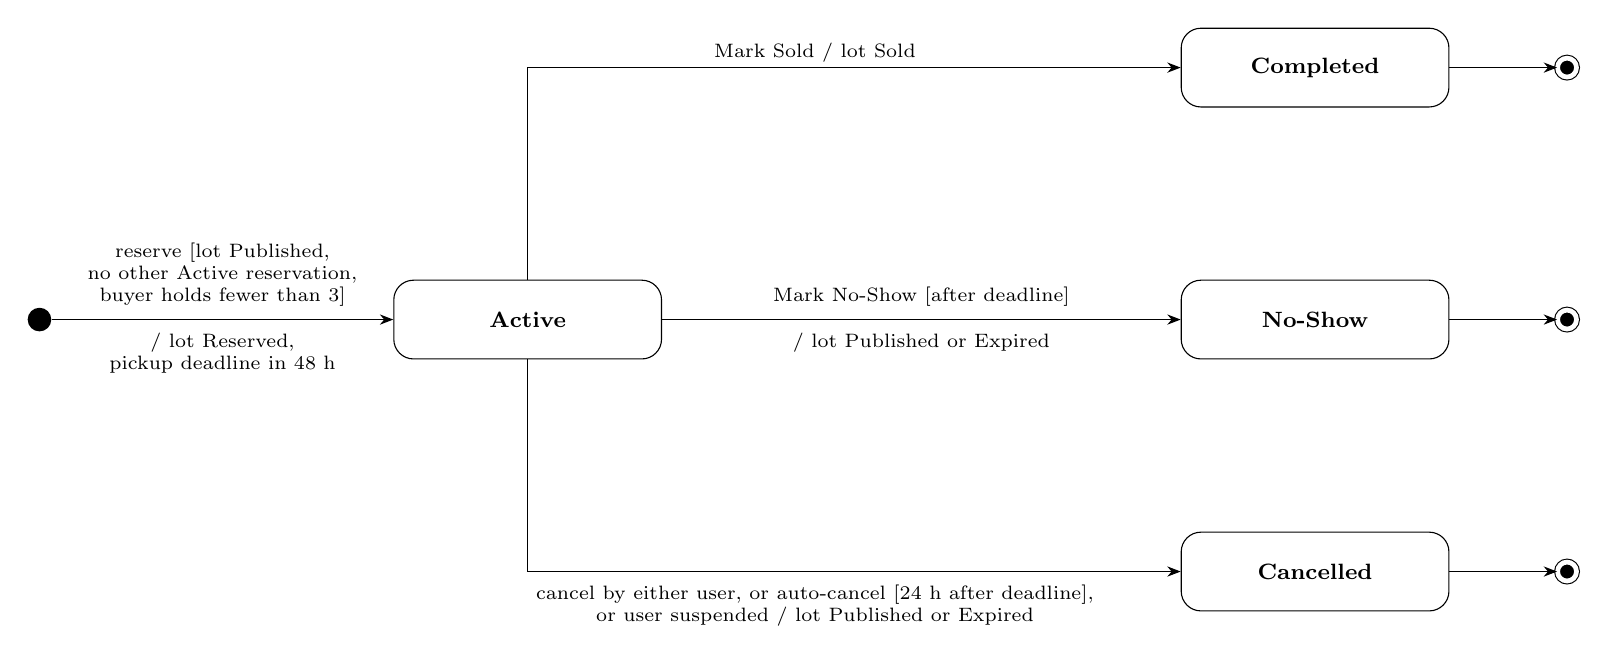
\begin{tikzpicture}[diagram]
  \node[ad initial] (i) at (-62,0) {};
  \node[st] (act) at (0,0) {Active};
  \node[st] (com) at (100,32) {Completed};
  \node[st] (nos) at (100,0) {No-Show};
  \node[st] (can) at (100,-32) {Cancelled};
  \node[ad final] (f1) at (132,32) {};
  \node[ad final] (f2) at (132,0) {};
  \node[ad final] (f3) at (132,-32) {};
  \draw[->] (i) -- node[tl,above=1mm]{reserve [lot Published,\\no other Active reservation,\\buyer holds fewer than 3]}node[tl,below=1mm]{/ lot Reserved,\\pickup deadline in 48 h} (act);
  \draw[->] (act.north) |- node[tl,pos=.72,above]{Mark Sold / lot Sold} (com.west);
  \draw[->] (act) -- node[tl,above=1mm]{Mark No-Show [after deadline]}node[tl,below=1mm]{/ lot Published or Expired} (nos);
  \draw[->] (act.south) |- node[tl,pos=.72,below=1mm]{cancel by either user, or auto-cancel [24 h after deadline],\\or user suspended / lot Published or Expired} (can.west);
  \draw[->] (com) -- (f1);
  \draw[->] (nos) -- (f2);
  \draw[->] (can) -- (f3);
\end{tikzpicture}
\end{document}
